\providecommand{\main}{..}
\documentclass[\main/main.tex]{subfiles}

\begin{document}
\graphicspath{{img/}{05_software/img/}}

\chapter{Software architecture}
\begin{figure}[H]
    \begin{center}
        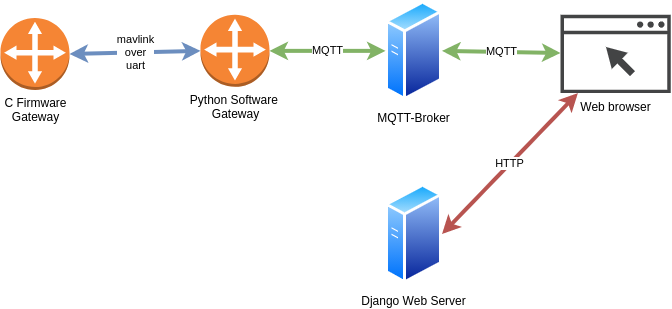
\includegraphics[width=0.9\textwidth]{software_architecture.png}
    \end{center}
    \caption{Software architecture}
    \label{fig:software_architecture}
\end{figure}
A system of software application is built to manage and control both the Bluetooth mesh network and the UWB ranging network. As represented in figure \ref{fig:software_architecture}, a gateway is built of two parts: a firmware application running in a microcontroller (e.g. nRF52832) written in C language and a software application running in an embedded computer (e.g. BeagleBone Green Wireless) written in Python language. There is an  MQTT-Broker (e.g. Eclipse Mosquitto) and a Django-based server running in the embedded computer too. This chapter provides a brief introduction to the structure of each component together with  the protocol manipulated to communicate between such components.

\section{Gateway firmware}
The main role of gateway firmware is to convert Bluetooth mesh messages to MAVLink messages and vice versa. As illustrated in figure \ref{fig:gateway_firmware}, four threads run in the gateway firmware. The net receiver thread listens for MAVLink messages and puts them into the mav2mesh\_mqueue message queue. The OS notifies the mesh sender thread when messages are available in the message queue. The mesh sender thread then sends it to the mesh network. The process is reserved for the message from the mesh network. As each message put to the message queue is a struct, threads must convert from theirs received message type to an application well-known struct before giving it to the message queue.

\begin{figure}[H]
    \begin{center}
        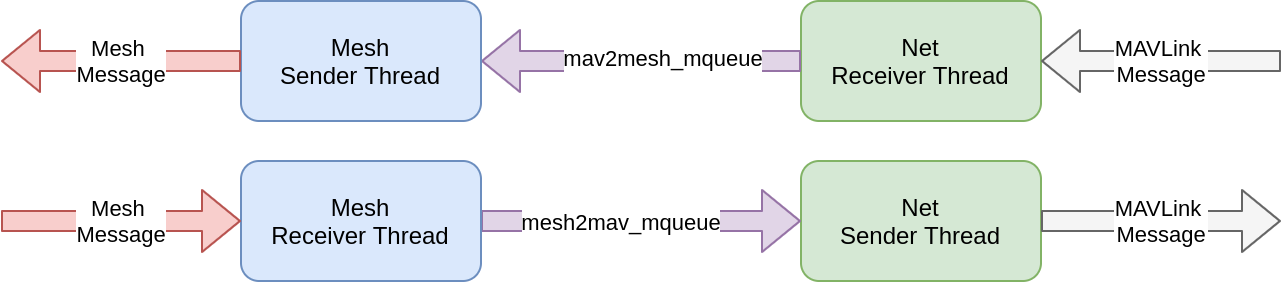
\includegraphics[width=0.9\textwidth]{gateway_firmware.png}
    \end{center}
    \caption{Gateway firmware component}
    \label{fig:gateway_firmware}
\end{figure}

The firmware part and software part of the gateway exchange messages using MAVLink/UART communication model as shown in figure \ref{fig:software_architecture}. The detailed description for this is provided in the following section.

\section{MAVLink over UART}
The layered architecture for the MAVLink/UART communication model is illustrated in figure \ref{fig:mavlink_uart_stack}.
\begin{figure}[H]
    \begin{center}
        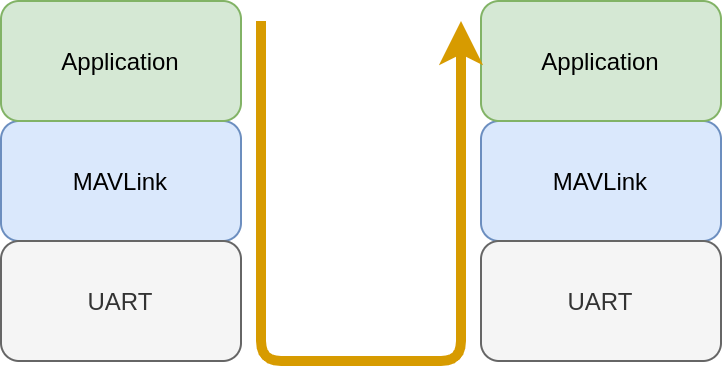
\includegraphics[width=0.5\textwidth]{MAVLink_over_UART.png}
    \end{center}
    \caption{MAVLink/UART stack}
    \label{fig:mavlink_uart_stack}
\end{figure}

\subsection{What is MAVLink?}
MAVLink is a very lightweight messaging protocol for communicating with drones and between onboard drone components \cite{web_mavlink}.

\subsection{MAVLink packet format}

Figure \ref{fig:packet_mavlink_v1} is the over-the-wire format for a MAVLink 1 packet, the in-memory representation might differ.

The minimum packet length is 8 bytes for acknowledgment packets without payload.

The maximum packet length is 263 bytes for full payload.

Explanation for each field in the MAVLink V1 frame is given in table \ref{tab:mavlink_v1_frame_explanation}.
\begin{figure}[H]
    \begin{center}
        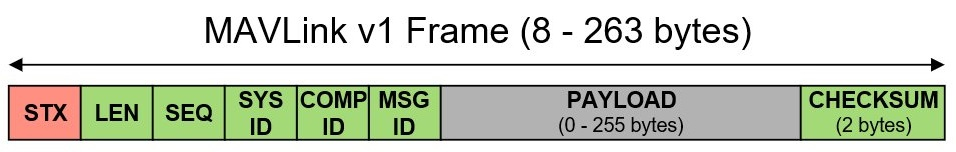
\includegraphics[width=0.9\textwidth]{packet_mavlink_v1.jpg}
    \end{center}
    \caption{MAVLink packet v1}
    \label{fig:packet_mavlink_v1}
\end{figure}

\begin{table}[H]
    \begin{tabular}{ | p{1.3cm} | p{1.8cm} | p{2cm} | l | p{9cm} |}
    \hline
    Byte Index & C version & Content & Value & Explanation \\\hline
    0 & uint8\_t magic & Packet start marker	& 0xFD & Protocol-specific start-of-text (STX) marker used to indicate the beginning of a new packet. Any system that does not understand protocol version will skip the packet. \\\hline
    1 & uint8\_t len & Payload length & 0 - 255	& Indicates length of the following payload section. This may be affected by payload truncation. \\\hline
    2 & uint8\_t seq	& Packet sequence number & 0 - 255 & Used to detect packet loss. Components increment value for each message sent. \\\hline
    3 & uint8\_t sysid & System ID & 1 - 255 & ID of system  sending the message. Used to differentiate systems on network.\\\hline
    4 & uint8\_t compid	& Component ID & 1 - 255 & ID of component sending the message. Used to differentiate components in a system. \\\hline
    5 & uint8\_t msgid & Message ID & 0 - 255 & ID of message type in payload. Used to decode data back into message object.\\\hline
    \end{tabular}
    \caption{MAVLink V1 frame explanation}
    \label{tab:mavlink_v1_frame_explanation}
\end{table}

\subsection{Pymavlink}

This is a Python implementation of the MAVLink protocol. It includes a source code generator (generator/mavgen.py) to create MAVLink protocol implementations for other programming languages as well. 

Figure \ref{net_mesh_mavlink_protocol} shows an example definition for message exchanged between gateway firmware and software. The \textbf{mavgen.py} script is used to generate C and Python implementation for the protocol from the XML file given in figure \ref{net_mesh_mavlink_protocol}. The C implementation is used in firmware while the Python one is used in software.

\section{Gateway software}
Similar to the gateway firmware, the main role of gateway software is to convert from MAVLink messages to JSON format strings, publish them to an MQTT topic and vice versa. Fortunately, the generated Python implementation provides APIs to easily convert a MAVLink message to a JSON string. As represented in figure \ref{fig:gateway_software}, two threads run in the software application play the opposite role. 

\begin{figure}[H]
    \begin{lstlisting}[style=XMLStyle, emph={messages, message, enums, enum, mavlink}]
<?xml version="1.0"?>
<mavlink>
    <version>3</version>

    <enums>
        <enum name="role_t">
            <entry name="ANCHOR"></entry>
            <entry name="TAG"></entry>
        </enum>
    </enums>

    <messages>
        <message id="0" name="BLINK">
            <description>Location message</description>
            <field type="uint16_t" name="uwb_address"/>
            <field type="uint8_t" enum="role_t" name="role"/>
        </message>
        <message id="2" name="ONOFF">
            <description>On off message</description>
            <field type="uint16_t" name="uwb_address"/>
            <field type="uint8_t" name="value"/>
        </message>
        <message id="4" name="LOCATION_REDUCED">
            <description>Location message</description>
            <field type="uint16_t" name="mesh_address"/>
            <field type="float" name="location_x"/>
            <field type="float" name="location_y"/>
        </message>
        <message id="7" name="SLOT">
            <description>Slot message</description>
            <field type="uint16_t" name="uwb_address"/>
            <field type="uint8_t" name="slot"/>
        </message>
    </messages>
</mavlink>
    \end{lstlisting}
    \caption{XML definition for message exchanged between firmware and software}
    \label{net_mesh_mavlink_protocol}
\end{figure}

\begin{figure}[H]
    \begin{center}
        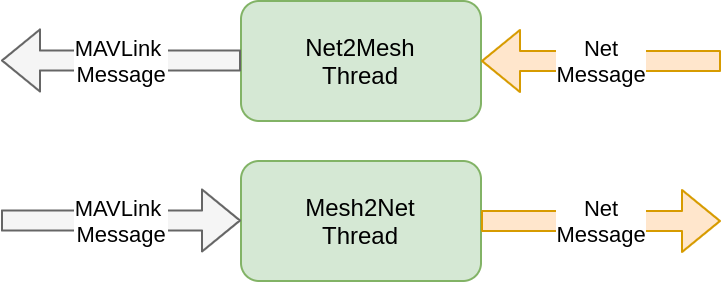
\includegraphics[width=0.5\textwidth]{gateway_software.png}
    \end{center}
    \caption{Gateway software component}
    \label{fig:gateway_software}
\end{figure}

\section{MQTT}
MQTT is an OASIS standard messaging protocol for the Internet of Things (IoT). It is designed as an extremely lightweight publish/subscribe messaging transport that is ideal for connecting remote devices with a small code footprint and minimal network bandwidth. MQTT today is used in a wide variety of industries, such as automotive, manufacturing, telecommunications, oil and gas, etc \cite{web_mqtt_org}.

MQTT protocol works on top of TCP/IP protocol and uses port 1883 (8883 if connecting through SSL) as default.
\begin{figure}[H]
    \begin{center}
        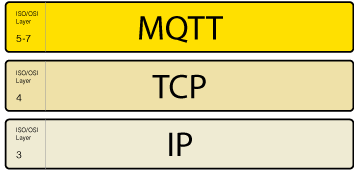
\includegraphics[width=0.3\textwidth]{mqtt_tcp.png}
    \end{center}
    \caption{MQTT layer in OSI model}
    \label{fig:mqtt_tcp}
\end{figure}

\subsection{Why MQTT?}

There are a number of reasons answering the question: Why MQTT is widely used in IOT? 
\begin{itemize}
    \item \textbf{Lightweight and efficient}: MQTT clients are very small, require minimal resources so can be used on small microcontrollers. MQTT message headers are small to optimize network bandwidth.
    \item \textbf{Bi-directional communications}: MQTT allows for messaging between device to cloud and cloud to device. This makes for easy broadcasting messages to groups of things.
    \item \textbf{Scale to millions of things}: MQTT can scale to connect with millions of IoT devices.
    \item \textbf{Reliable message delivery}: Reliability of message delivery is important for many IoT use cases. This is why MQTT has 3 defined quality of service levels: 0 - at most once, 1- at least once, 2 - exactly once
    \item \textbf{Support for unreliable networks}: Many IoT devices connect over unreliable cellular networks. MQTT’s support for persistent sessions reduces the time to reconnect the client with the broker.
    \item \textbf{Security enabled}: MQTT makes it easy to encrypt messages using TLS and authenticate clients using modern authentication protocols, such as OAuth.
\end{itemize}

\subsection{MQTT publish/subscribe architecture}
The Publisher sends data on the MQTT Broker specifying a definite topic in a message. The Subscribers can receive various data from multiple Publishers depending on subscription to correspondent topics.
\begin{figure}[H]
    \begin{center}
        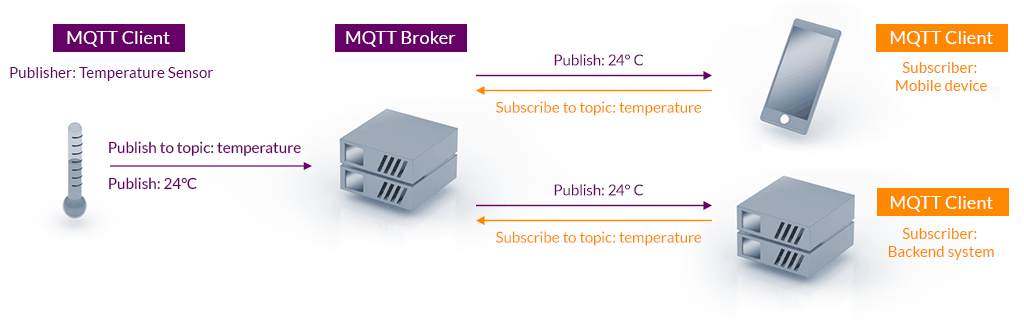
\includegraphics[scale=0.35]{mqtt-publish-subscribe.png}
    \end{center}
    \caption{MQTT publish subscribe}
    \label{fig:mqtt_publish_subscribe.}
\end{figure}

Here are the main types of messages for an MQTT device to communication with the Broker:

\begin{itemize}
    \item Connect: establish the connection to the Broker
    \item Disconnect: break the connection to the Broker
    \item Publish: publish data on a topic within the message Broker
    \item Subscribe: subscribe to a topic on the message Broker
    \item Unsubscribe: unsubscribe the topic
\end{itemize}


Figure \ref{fig:mqtt_schema} illustrates a scheme of simple communication between subscriber, publisher and broker: 
\begin{figure}[H]
    \begin{center}
        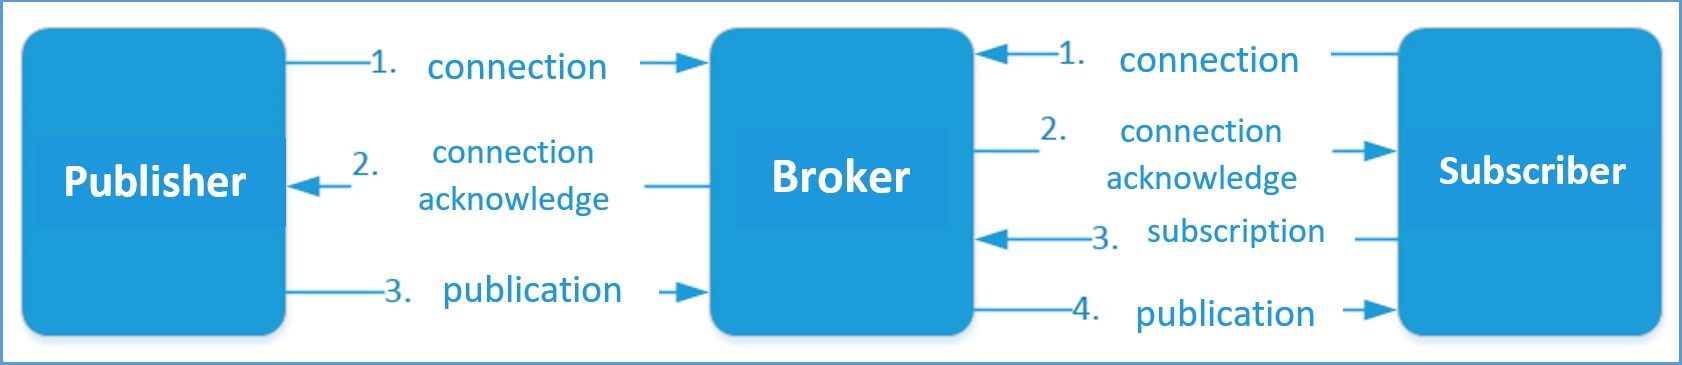
\includegraphics[width=0.8\textwidth]{mqtt_schema.jpg}
    \end{center}
    \caption{MQTT simple scheme}
    \label{fig:mqtt_schema}
\end{figure}

\subsection{Quality of service in MQTT protocol (QoS)}

MQTT supports three levels of Quality of Service (QoS) when sending messages.

\subsubsection{QoS 0: At most once}
This service level guarantees a best-effort delivery. There is no guarantee of delivery. The recipient does not acknowledge receipt of the message and the message is not stored and re-transmitted by the sender. QoS level 0 is often called “fire and forget” and provides the same guarantee as the underlying TCP protocol.
\begin{figure}[H]
    \begin{center}
        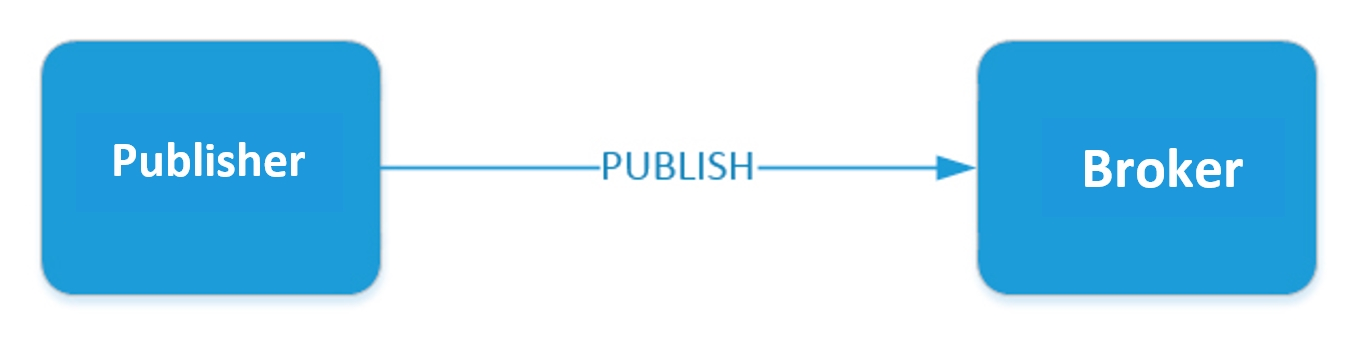
\includegraphics[width=0.6\textwidth]{mqtt_qos_0.jpg}
    \end{center}
    \caption{QoS 0: At most once}
    \label{fig:mqtt_qos_0}
\end{figure}

\subsubsection{QoS 1: At least once}
This level guarantees the message delivery to the broker, however, the duplication of messages from the publisher is possible. Once a duplicate copy is received, the broker sends out this message to the subscribers again, and forwards the message receipt acknowledgment to the publisher. If the publisher does not get PUBACK message from the broker, it will attempt to re-deliver this packet.

\begin{figure}[H]
    \begin{center}
        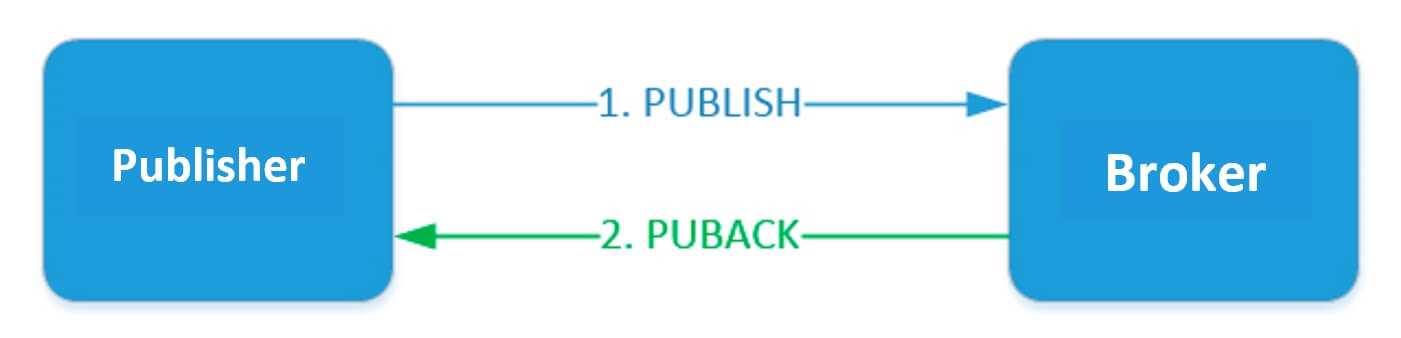
\includegraphics[width=0.6\textwidth]{mqtt_qos_1.jpg}
    \end{center}
    \caption{QoS 1: At least once}
    \label{fig:mqtt_qos_1}
\end{figure}

\subsubsection{QoS 2: Exactly once}
On this level the message delivery to a Client is guaranteed, with no duplication copies possible.

\begin{figure}[H]
    \begin{center}
        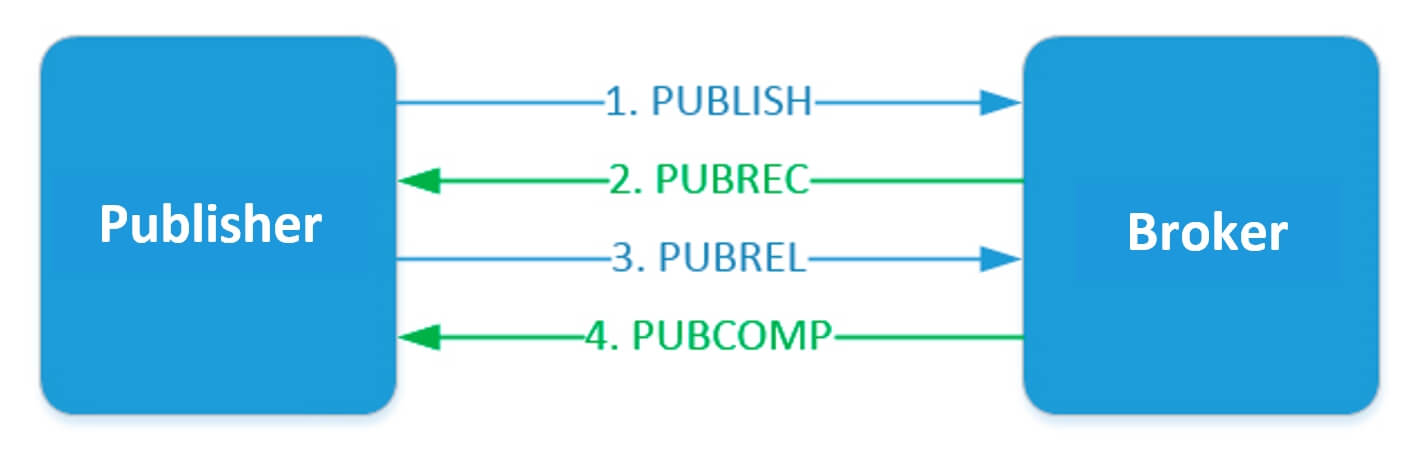
\includegraphics[width=0.6\textwidth]{mqtt_qos_2.jpg}
    \end{center}
    \caption{QoS 2: Exactly once}
    \label{fig:mqtt_qos_2}
\end{figure}
The publisher sends a message to the broker. The message contains the unique packet ID, QoS=2 and DUP=0. The publisher stores the message unacknowledged unless it gets a PUBREC response from the broker. The broker replies with the PUBREC message containing the same packet ID. After receiving this message, the publisher sends PUBREL with the same packet ID. The broker must store the message copy until it gets PUBREL. Once the broker receives PUBREL, it deletes the message copy and sends to the publisher the PUBCOMP message about the completed transaction.

\subsection{MQTT application message definition}
The application message transferred over the MQTT connection is derived from the protocol XML file as illustrated in figure \ref{fig:gateway_software}. The generated Python implementation automatically provides APIs for converting MAVLink messages to JSON strings.  These JSON strings are then published to an MQTT topic as shown in figure \ref{fig:mqtt_json_string}.

\begin{figure}[H]
    \begin{center}
        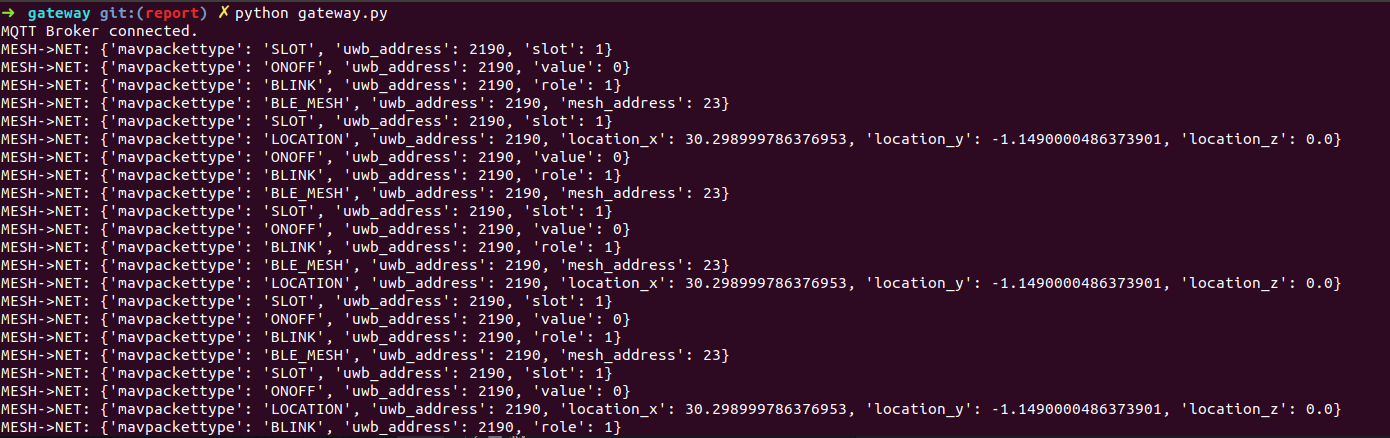
\includegraphics[width=0.95\textwidth]{mqtt_json_string.png}
    \end{center}
    \caption{MQTT json string}
    \label{fig:mqtt_json_string}
\end{figure}

\section{System control and management application}
Figure \ref{fig:system_control_and_manage_application} provides an overview for the GUI used control and manage the ranging network.
\begin{figure}[H]   
    \centering
    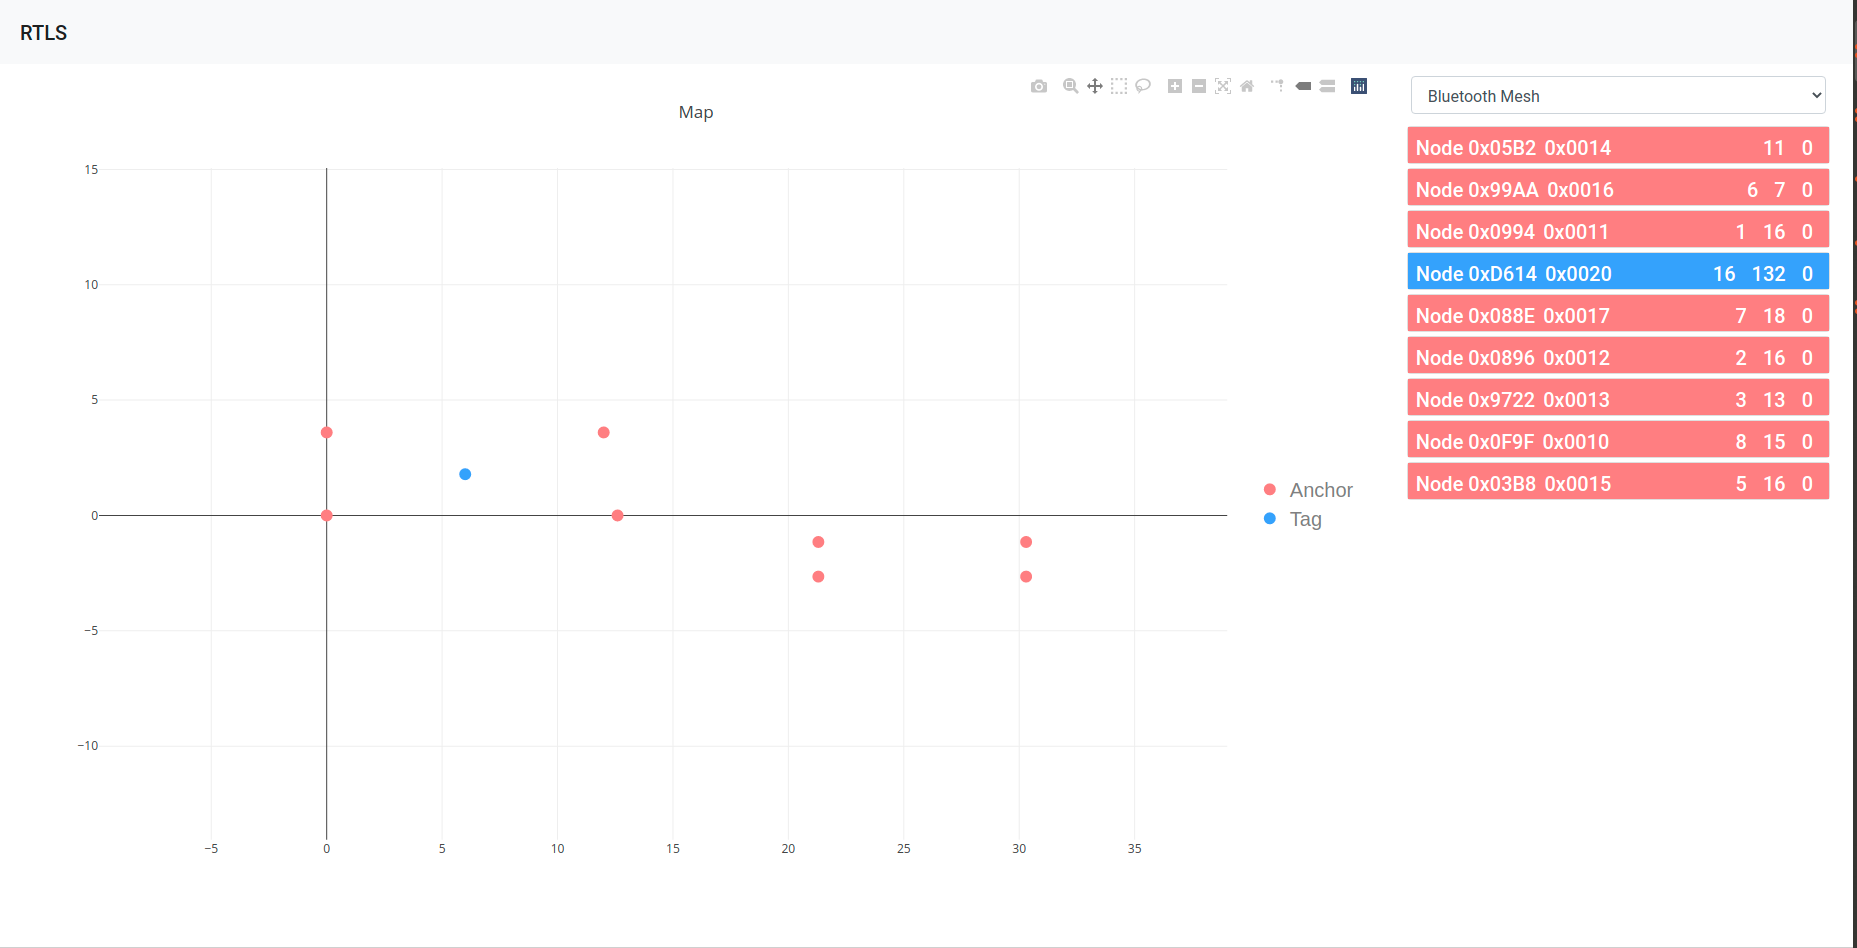
\includegraphics[width=1\textwidth]{system_control_and_manage_application.png}
    \caption{System control and manage application}
    \label{fig:system_control_and_manage_application}
\end{figure}
As shown in figure \ref{fig:system_control_and_manage_application}, there are two main part in the GUI. The left part is a simple map which give a quick illustration for the location of tags and anchors. The right part is a list of nodes available in the system. Detailed information of each items in the list is given in figure \ref{fig:control_and_manage_pannel}

\begin{figure}[H]   
    \centering
    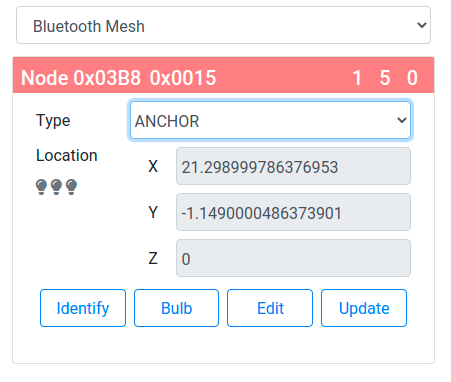
\includegraphics[width=0.5\textwidth]{control_and_manage_pannel.png}
    \caption{Node panel}
    \label{fig:control_and_manage_pannel}
\end{figure}

Below are the descriptions for each field:
\begin{itemize}
    \item The field with the value of 0x03B8: The address of the node in UWB network
    \item The field with the value of 0x0015: The address of the node in Bluetooth mesh network
    \item The field with the value of 1: The slot index of the node in the TDMA network
    \item The field with the value of 5: The number of location messages received by the application.
    \item The field with the value of 0: The number of on-off messages received by the application.
    \item Type: The type of the node: ANCHOR or TAG
    \item Location: The location of the node
    \item Identify button: Turn on/off the self-identification process of the node
    \item Bulb button: Turn on/off light bulb on the anchor
    \item Edit button: Enter the editing mode to change node type and location (location edit is only available for anchor)
    \item Update button: Update the configuration (node type and location) to the node, only available in editing mode
\end{itemize}

\bib

\end{document}